% This must be in the first 5 lines to tell arXiv to use pdfLaTeX.
\pdfoutput=1
\documentclass[11pt]{article}
\usepackage[]{ACL2023}
\usepackage{times}
\usepackage{latexsym}
\usepackage{graphicx}
\usepackage{amsmath}
\usepackage{amssymb}
\usepackage{hyperref}
\usepackage[T1]{fontenc}
\usepackage[utf8]{inputenc}
\usepackage{microtype}
\usepackage{inconsolata}
\usepackage{booktabs}
\usepackage{multirow}

\setlength\titlebox{6cm}

\title{Violence Event Detection and Temporal Localization in Surveillance Video: \\
A Weakly-Supervised Multi-Dataset Framework \\
{\large Milestone 2: Baseline Reproduction and Early Solution Results}}

\author{
Srinivasa Sai Chava \\
Boston University \\
\texttt{saichava@bu.edu}
\And
Shrishty Gupta \\
Boston University \\
\texttt{shrishty@bu.edu}
\And
Vishakha \\
Boston University \\
\texttt{vish1909@bu.edu}
\AND
Anagha \\
Boston University \\
\texttt{anaghapk@bu.edu}
\And
Yuxiang Liu \\
Boston University \\
\texttt{mat1900@bu.edu}
}

\begin{document}
\maketitle

\begin{abstract}
Traditional video anomaly detection treats surveillance as binary classification, producing coarse video-level predictions without event identity or temporal boundaries. We propose a weakly-supervised framework specifically for \textbf{violence event detection and temporal localization}, focusing on 6 violence categories with strong cross-dataset support. Our method operates on pre-extracted I3D features (not end-to-end training) and combines Multiple Instance Learning with a Temporal Refinement Network. We evaluate on 4 datasets: UCF-Crime (primary, 6 violence categories), XD-Violence (transfer, 4 overlapping categories), RWF-2000 (fight validation), and ShanghaiTech (robustness). \textbf{Milestone 2 status:} dataset preparation is complete (1,300 videos, all features extracted), the RTFM baseline has been reproduced (AUC~0.9213), and an early solution with a Temporal Refinement Network shows improved AP (0.8663 vs.\ 0.8290 baseline).
\end{abstract}

% -------------------------------------------------------
% SECTION 1 — INTRODUCTION (kept for context)
% -------------------------------------------------------
\section{Introduction}
Video surveillance systems face a critical gap: while automated anomaly detection has improved, most methods output only binary predictions without identifying \textit{what} happened and \textit{when}. For security operations, violence detection is the highest-priority anomaly class, motivating our focus.

\textbf{Research Question:} Can we detect, classify, and temporally localize violence events in surveillance video using only video-level labels, and how well does this generalize across different datasets and environments?

We focus specifically on \textbf{violence event detection} (6 categories: Fighting, Shooting, Explosion, Robbery, Abuse, Riot). Our approach combines MIL-based anomaly scoring with a Temporal Refinement Network (TRN) and a boundary head, trained on weakly-labeled UCF-Crime data using frozen I3D features.

% -------------------------------------------------------
% SECTION 2 — RELATED WORK (kept for context)
% -------------------------------------------------------
\section{Related Work}

\subsection{Weakly-Supervised Video Anomaly Detection}
Sultani et al.\ \cite{sultani2018real} pioneered weakly-supervised VAD using MIL on UCF-Crime with pre-extracted C3D features. RTFM \cite{tian2021weakly} improved this using I3D features and feature magnitude learning. Both methods use pre-extracted features rather than end-to-end training, validating our design choice.

Recent work addresses score instability and noisy labels (DSS, DAKD \cite{lan2025dss, wang2025dakd}), event-completeness modeling (LEC-VAD \cite{tian2025lecvad}), and category-aware routing (GS-MoE \cite{wang2025gsmoe}).

\subsection{Violence Detection and Temporal Localization}
XD-Violence \cite{wu2020not} introduced multi-modal violence detection. Transformer-based methods \cite{wu2023surveillance} improve temporal representations. Fully-supervised temporal localization methods (ActionFormer \cite{zhang2022actionformer}, TriDet \cite{shi2023tridet}) achieve high precision but require expensive frame-level annotations --- our weakly-supervised setting avoids this requirement.

% -------------------------------------------------------
% SECTION 3 — METHODOLOGY (kept: describes what was built)
% -------------------------------------------------------
\section{Methodology}

\subsection{Problem Formulation}
\textbf{Input:} Untrimmed video $V$ divided into $T$ non-overlapping 16-frame segments, each represented as a frozen I3D feature $f_t \in \mathbb{R}^{2048}$.

\textbf{Training supervision (weak):} video-level binary label $y \in \{0,1\}$ and category label $c \in \{1,\ldots,6\}$ for anomalous videos. No segment-level or boundary annotations.

\textbf{Output (per segment):} anomaly score $s_t \in [0,1]$, class distribution $p_t \in \mathbb{R}^6$, boundary confidence $b_t \in [0,1]$.

\subsection{Architecture}

Table~\ref{tab:params} shows the trainable parameter budget. The I3D backbone is kept frozen throughout.

\begin{table}[h]
\centering
\small
\begin{tabular}{lrr}
\toprule
\textbf{Component} & \textbf{Params} & \textbf{Trainable?} \\
\midrule
I3D Backbone     & 25M   & \textbf{No (frozen)} \\
MIL Scorer       & 1.3M  & Yes \\
Event Classifier & 400K  & Yes \\
TRN Module       & 500K  & Yes \\
Boundary Head    & 200K  & Yes \\
\midrule
\textbf{Total Trainable} & \textbf{2.4M} & \\
\bottomrule
\end{tabular}
\caption{Model architecture and trainable parameter budget.}
\label{tab:params}
\end{table}

\subsubsection{MIL Anomaly Scorer}
\begin{equation}
h^{(1)}_t = \text{ReLU}(W_1 f_t + b_1), \quad
h^{(2)}_t = \text{Dropout}(\text{ReLU}(W_2 h^{(1)}_t + b_2)), \quad
s_t = \sigma(w_3^\top h^{(2)}_t + b_3)
\end{equation}
Video-level score: $s_\text{video} = \text{mean}(\text{top-}k \text{ segments})$, $k = \lceil T \cdot 0.125 \rceil$.

\subsubsection{Classifier Branch}
Top-$k$ segments per anomalous video receive pseudo-labels matching the video's category. Loss:
\begin{equation}
\mathcal{L}_{cls} = -\frac{1}{|P|} \sum_{t \in P} \log p_t[c_\text{video}]
\end{equation}

\subsubsection{Temporal Refinement Network (TRN)}
A 2-layer transformer encoder (4 heads, FFN dim 2048, learned positional encoding, dropout 0.1) refines segment representations using full temporal context before anomaly scoring and classification.

\subsubsection{Boundary Head}
\begin{equation}
b_t = \sigma\!\left(W_b\, [\tilde{h}_t\,;\,\tilde{h}_{t+1}\,;\,|\tilde{s}_t - \tilde{s}_{t+1}|] + b_b\right)
\end{equation}

\subsection{Training Objective}
\begin{equation}
\mathcal{L} = \mathcal{L}_\text{MIL} + 0.5\,\mathcal{L}_{cls} + 0.3\,\mathcal{L}_{bnd} + 0.1\,\mathcal{L}_{smooth}
\end{equation}

% -------------------------------------------------------
% COMMENTED OUT: Work Division, Timeline, Success Criteria
% (proposal logistics — not relevant to Milestone 2 results)
% \section{Work Division} ...
% \section{Timeline} ...
% \section{Success Criteria} ...
% -------------------------------------------------------

% -------------------------------------------------------
% MILESTONE 2 RESULTS — NEW SECTIONS
% -------------------------------------------------------

\section{Milestone 2: Dataset Preparation and Feature Extraction}

\subsection{UCF-Crime Violence Subset}
We built the primary training dataset from UCF-Crime selecting 5 violence categories (Fighting, Shooting, Explosion, Robbery, Abuse) plus Normal. The final manifest contains 1,300 videos with zero missing or corrupt files.

\begin{table}[h]
\centering
\small
\begin{tabular}{lrrrr}
\toprule
\textbf{Class} & \textbf{Train} & \textbf{Val} & \textbf{Test} & \textbf{Total} \\
\midrule
Fighting   &  41 &  4 &  5 &   50 \\
Shooting   &  24 &  3 & 23 &   50 \\
Explosion  &  26 &  3 & 21 &   50 \\
Robbery    & 131 & 14 &  5 &  150 \\
Abuse      &  43 &  5 &  2 &   50 \\
Normal     & 720 & 80 & 150 &  950 \\
\midrule
\textbf{Total} & \textbf{985} & \textbf{109} & \textbf{206} & \textbf{1,300} \\
\bottomrule
\end{tabular}
\caption{UCF-Crime violence subset: videos per class and split. All 206 test videos carry temporal boundary annotations.}
\label{tab:dataset_splits}
\end{table}

\textbf{Class imbalance note:} Robbery dominates (150 total vs.\ 50 for other violence classes), and abuse has only 2 test videos. This limits macro-F1 reliability for small classes and is a known reporting constraint.

\subsection{I3D Feature Extraction}

\begin{itemize}
\item \textbf{Extractor:} pytorchvideo \texttt{i3d\_r50}, Kinetics-400 pretrained.
\item \textbf{Feature layer:} pooled penultimate embedding (classification head removed), $D = 2048$.
\item \textbf{Segment policy:} non-overlapping 16-frame chunks; leftover frames ($< 16$) dropped.
\item \textbf{Input:} shorter-side resize 256, center crop $224\!\times\!224$, Kinetics normalization.
\item \textbf{Backbone state:} frozen throughout (inference only).
\end{itemize}

\textbf{Result:} 1,300/1,300 videos extracted successfully, 0 failures. Each video saved as \texttt{.npz} array of shape $[T, 2048]$ where $T = \lfloor N_\text{frames} / 16 \rfloor$.

\begin{table}[h]
\centering
\small
\begin{tabular}{lrrrr}
\toprule
\textbf{Split} & \textbf{Min $T$} & \textbf{Max $T$} & \textbf{Mean $T$} & \textbf{Median $T$} \\
\midrule
Train &  12 & 61,031 & 631 & 140 \\
Val   &  15 &  5,476 & 358 & 169 \\
Test  &  13 &  6,749 & 246 & 109 \\
\bottomrule
\end{tabular}
\caption{Segment count statistics per split ($T$ = 16-frame segments per video).}
\label{tab:feature_stats}
\end{table}

For training, sequences are uniformly sampled to 32 segments if longer, or padded by repeating the last segment if shorter, giving fixed-shape batches $[B, 32, 2048]$.

\section{Milestone 2: Baseline Reproduction (RTFM)}

Since we use a different data split (UCF-Crime violence subset only, 5 classes) and a different I3D extractor (pytorchvideo \texttt{i3d\_r50}) compared to the original RTFM paper, we reproduced the baseline rather than reporting the paper's numbers.

\subsection{Setup}

\textbf{Architecture:} feature projection $2048 \!\to\! 512$; scoring head $512 \!\to\! 256 \!\to\! 1$; top-$k$ aggregation ($k = \lceil T \cdot 0.125 \rceil$).

\textbf{Training:} $\mathcal{L} = \mathcal{L}_\text{BCE} + 0.1\,\mathcal{L}_\text{RTFM}$; Adam, lr $= 10^{-4}$, batch 64, 30 epochs; checkpoint by best validation AUC.

\subsection{Results}

\begin{table}[h]
\centering
\small
\begin{tabular}{lr}
\toprule
\textbf{Metric} & \textbf{Value} \\
\midrule
Test AUC           & 0.9213 \\
Test AP            & 0.8290 \\
\midrule
\multicolumn{2}{l}{\textit{Confusion matrix @ threshold 0.5}} \\
True Negative  (normal correct)    & 139 \\
False Positive (normal as anomaly) &  11 \\
False Negative (anomaly missed)    &  17 \\
True Positive  (anomaly correct)   &  39 \\
\midrule
Best val epoch (of 30) & 18 \\
Val AUC @ best epoch   & 0.9759 \\
\bottomrule
\end{tabular}
\caption{RTFM baseline test results on UCF-Crime violence subset (206 test videos).}
\label{tab:baseline_results}
\end{table}

\subsubsection{Training Curves}
Figure~\ref{fig:step4_curves} shows stable convergence with no overfitting. Training loss drops from 1.1 to 0.22 over 30 epochs. Validation AUC rises sharply in the first 8 epochs and plateaus at 0.975, confirming the model is not overfitting to the training set.

\begin{figure}[h]
\centering
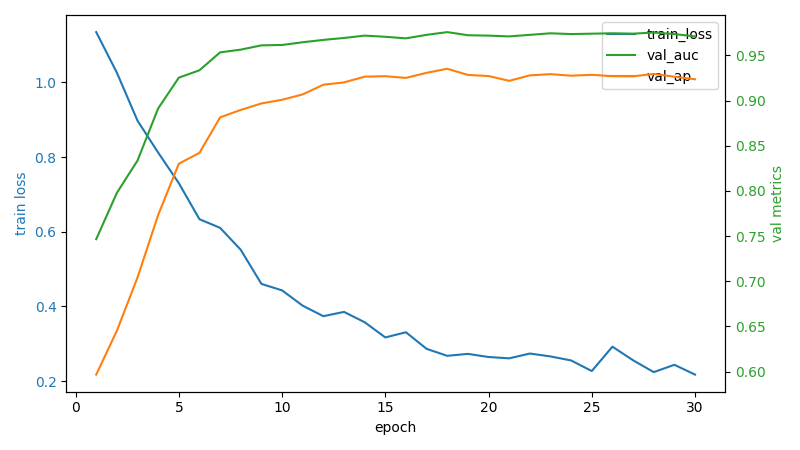
\includegraphics[width=\columnwidth]{figures/step4_train_curves.png}
\caption{RTFM baseline: training loss (left axis) and validation AUC/AP (right axis) over 30 epochs. Best checkpoint selected at epoch 18.}
\label{fig:step4_curves}
\end{figure}

\subsubsection{Score Distribution Analysis}

Figure~\ref{fig:score_hist} shows the video-level anomaly score distribution for normal and anomaly videos on the test set. Table~\ref{tab:score_dist} gives the summary statistics.

\begin{figure}[h]
\centering
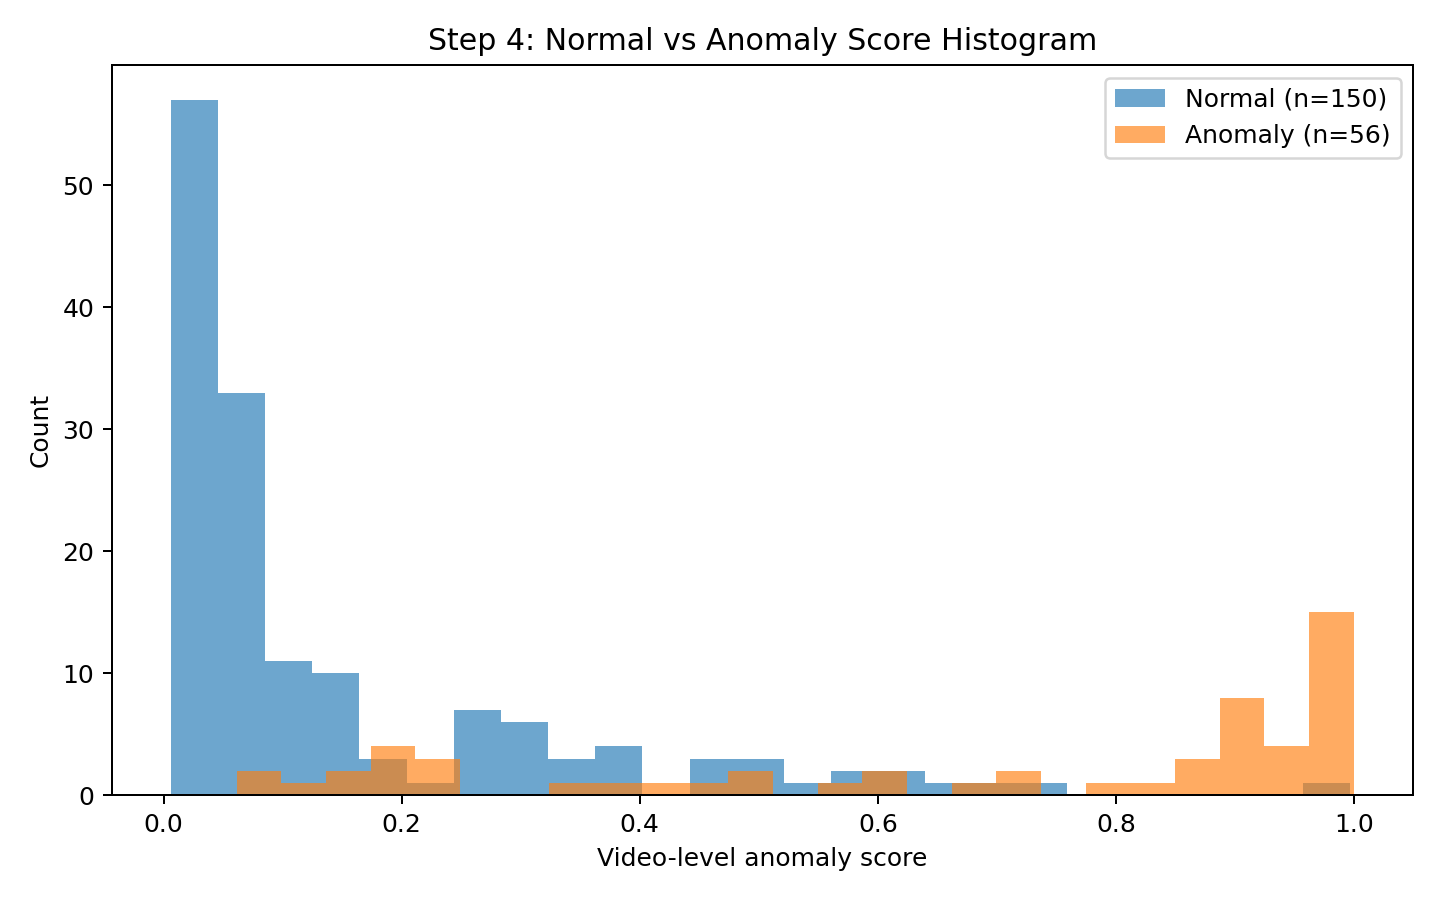
\includegraphics[width=\columnwidth]{figures/milestone2_score_hist.png}
\caption{Normal vs.\ anomaly score histogram (test set, 206 videos). Normal scores concentrate near 0; anomaly scores are bimodal --- a cluster near 1.0 (Explosion, Shooting) and a low cluster near 0 (Abuse).}
\label{fig:score_hist}
\end{figure}

\begin{table}[h]
\centering
\small
\begin{tabular}{lrrrrrr}
\toprule
\textbf{Group} & \textbf{N} & \textbf{Mean} & \textbf{Median} & \textbf{Q25} & \textbf{Q75} & \textbf{Max} \\
\midrule
Normal  & 150 & 0.148 & 0.062 & 0.036 & 0.169 & 0.997 \\
Anomaly &  56 & 0.689 & 0.870 & 0.411 & 0.971 & 1.000 \\
\bottomrule
\end{tabular}
\caption{Score distribution statistics for normal vs.\ anomaly test videos. Anomaly median (0.870) is well separated from normal median (0.062), explaining the AUC of 0.9213.}
\label{tab:score_dist}
\end{table}

\textbf{Key observation:} The anomaly score distribution is bimodal. Visually distinct violence (Explosion, Shooting) clusters near 1.0, while subtle violence (Abuse) falls near the normal range. This matches the confusion matrix: most errors involve abuse videos being scored like normal ones.

\subsubsection{Hard Case Examples}

Table~\ref{tab:hard_cases} shows representative score examples illustrating the easy and hard ends of the test set.

\begin{table}[h]
\centering
\small
\begin{tabular}{llrr}
\toprule
\textbf{Video} & \textbf{Class} & \textbf{Score} & \textbf{Correct?} \\
\midrule
Normal\_Videos\_003 & normal    & 0.014 & \checkmark \\
Normal\_Videos\_015 & normal    & 0.033 & \checkmark \\
Normal\_Videos\_014 & normal    & 0.268 & \checkmark (marginal) \\
Normal\_Videos\_010 & normal    & 0.378 & \checkmark (marginal) \\
\midrule
Explosion002        & explosion & 0.990 & \checkmark \\
Explosion004        & explosion & 0.992 & \checkmark \\
Abuse030            & abuse     & 0.242 & \checkmark (marginal) \\
Abuse028            & abuse     & 0.183 & \texttimes\ (FN) \\
\bottomrule
\end{tabular}
\caption{Representative score examples from the test set. Marginal cases sit near the 0.5 threshold; FN = false negative.}
\label{tab:hard_cases}
\end{table}

\subsubsection{Qualitative Segment Ranking}

Table~\ref{tab:seg_ranking} shows which 16-frame segments the baseline assigns the highest anomaly scores to, for three representative test videos.

\begin{table}[h]
\centering
\small
\begin{tabular}{llp{3.2cm}r}
\toprule
\textbf{Video} & \textbf{Class} & \textbf{Top-3 frame ranges} & \textbf{Min score} \\
\midrule
Explosion021 & explosion & 192--207, 528--543, 496--511 & 0.997 \\
Shooting026  & shooting  & 528--543, 480--495, 576--591 & 0.999 \\
Explosion020 & explosion & 112--127, 160--175, 448--463 & 0.981 \\
\bottomrule
\end{tabular}
\caption{Top-3 high-scoring segments per video (frame ranges = 16-frame chunk boundaries). Scores $\geq 0.98$ across all top segments confirm the model localizes obvious violence events consistently.}
\label{tab:seg_ranking}
\end{table}

\section{Milestone 2: Early Solution Results (+ TRN)}

\subsection{Model Extensions}

Building on the baseline we added two components incrementally:

\textbf{Step 5 — Classifier branch:} 6-class head on scorer hidden features, trained with pseudo-labels (top-4 segments per anomalous video receive the video's category; all normal segments labeled ``normal'').

\textbf{Step 6 — Temporal Refinement Network:} 2-layer transformer encoder inserted between projection and prediction heads, providing temporal context across all 32 segments before scoring.

\subsection{Comparison}

\begin{table}[h]
\centering
\small
\begin{tabular}{lrrrr}
\toprule
\textbf{Model} & \textbf{AUC} & \textbf{AP} & \textbf{Macro-F1} & \textbf{W-F1} \\
\midrule
RTFM Baseline (Step 4)  & 0.9213 & 0.8290 & ---    & ---    \\
+ Classifier (Step 5)   & 0.9108 & 0.8305 & 0.2273 & 0.6833 \\
+ TRN (Step 6)          & 0.9096 & \textbf{0.8663} & \textbf{0.3543} & \textbf{0.7405} \\
\bottomrule
\end{tabular}
\caption{Progressive model comparison on UCF-Crime test set (206 videos). W-F1 = weighted F1.}
\label{tab:comparison}
\end{table}

\begin{figure}[h]
\centering
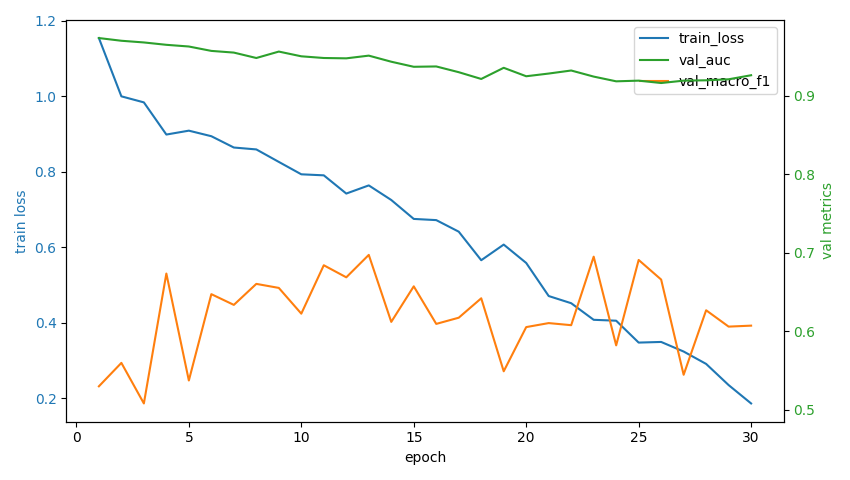
\includegraphics[width=\columnwidth]{figures/step6_train_curves.png}
\caption{Step 6 (TRN) training curves: loss and validation macro-F1/AUC over 30 epochs.}
\label{fig:step6_curves}
\end{figure}

\subsection{Per-Class Results (Step 6)}

\begin{table}[h]
\centering
\small
\begin{tabular}{lrrrr}
\toprule
\textbf{Class} & \textbf{Prec.} & \textbf{Recall} & \textbf{F1} & \textbf{Support} \\
\midrule
Normal    & 0.924 & 0.893 & 0.908 & 150 \\
Fighting  & 0.400 & 0.400 & 0.400 &   5 \\
Shooting  & 1.000 & 0.087 & 0.160 &  23 \\
Explosion & 0.571 & 0.381 & 0.457 &  21 \\
Robbery   & 0.120 & 0.600 & 0.200 &   5 \\
Abuse     & 0.000 & 0.000 & 0.000 &   2 \\
\midrule
\textbf{Macro avg} & & & \textbf{0.354} & 206 \\
\bottomrule
\end{tabular}
\caption{Per-class classification results for Step 6 (TRN) on UCF-Crime test set.}
\label{tab:perclass}
\end{table}

\subsection{Discussion}

\textbf{What improved:} AP increased from 0.8290 to 0.8663 (+4.5 pp) with TRN, indicating better violence segment ranking. Macro-F1 improved from 0.2273 (Step 5) to 0.3543 (+12.7 pp), showing that temporal context helps stabilize multi-class predictions. TRN attention weights are non-uniform (row-max mean 0.159 vs.\ uniform reference 0.031), confirming meaningful temporal dependencies are learned.

\textbf{What remains weak:} AUC dropped slightly (0.9213 $\to$ 0.9096) when adding classification supervision --- a known trade-off in MIL. Shooting recall is very low (0.087) due to class confusion with other violence types. Abuse F1 is 0 (only 2 test samples). The low macro-F1 is primarily driven by the highly imbalanced test set rather than a fundamental model failure.

\textbf{Next:} Full model (boundary head, progressive training, ablations, cross-dataset transfer) will be reported in Milestone 3.

% -------------------------------------------------------
% LIMITATIONS AND CONCLUSION
% -------------------------------------------------------
\section{Limitations}
\begin{itemize}
\item Violence-focused scope only; non-violence anomalies are excluded by design.
\item Weak supervision limits boundary precision; no segment-level labels are used.
\item Test set imbalance (e.g., 2 abuse, 5 robbery) makes macro-F1 unstable for small classes.
\item Cross-dataset evaluation constrained to overlapping categories.
\end{itemize}

\section{Conclusion}
At Milestone 2, the full UCF-Crime violence subset (1,300 videos) is prepared with frozen I3D features extracted for all videos. The RTFM baseline has been reproduced achieving AUC~0.9213. Adding a classifier branch and Temporal Refinement Network improves AP to 0.8663 and macro-F1 to 0.354. The full model with boundary head, progressive training, ablations, and cross-dataset evaluation will be reported in Milestones 3 and 4.

\bibliographystyle{acl_natbib}
\begin{thebibliography}{99}

\bibitem[Sultani et al.(2018)]{sultani2018real}
Waqas Sultani, Chen Chen, and Mubarak Shah.
\newblock 2018.
\newblock Real-world anomaly detection in surveillance videos.
\newblock In \textit{CVPR}, pages 6479--6488.

\bibitem[Tian et al.(2021)]{tian2021weakly}
Yu Tian, Guansong Pang, Yuanhong Chen, Rajvinder Singh, Johan W Verjans, and Gustavo Carneiro.
\newblock 2021.
\newblock Weakly-supervised video anomaly detection with robust temporal feature magnitude learning.
\newblock In \textit{ICCV}, pages 4975--4986.

\bibitem[Wu et al.(2020)]{wu2020not}
Peng Wu, Jing Liu, Yujia Shi, Yujia Sun, Fangtao Shao, Zhaoyang Wu, and Zhiwei Yang.
\newblock 2020.
\newblock Not only look, but also listen: Learning multimodal violence detection under weak supervision.
\newblock In \textit{ECCV}, pages 322--339.

\bibitem[Zhang et al.(2022)]{zhang2022actionformer}
Chen-Lin Zhang, Jianxin Wu, and Yin Li.
\newblock 2022.
\newblock ActionFormer: Localizing moments of actions with transformers.
\newblock In \textit{ECCV}, pages 492--510.

\bibitem[Shi et al.(2023)]{shi2023tridet}
Dingfeng Shi, Yujie Zhong, Qiong Cao, Lin Ma, Jia Li, and Dacheng Tao.
\newblock 2023.
\newblock TriDet: Temporal action detection with relative boundary modeling.
\newblock In \textit{CVPR}, pages 18857--18866.

\bibitem[Nguyen et al.(2018)]{nguyen2018weakly}
Phuc Xuan Nguyen, Deva Ramanan, and Charless C Fowlkes.
\newblock 2018.
\newblock Weakly-supervised action localization with background modeling.
\newblock In \textit{ICCV}, pages 5502--5511.

\bibitem[Paul et al.(2018)]{paul2018w}
Sujoy Paul, Sourya Roy, and Amit K Roy-Chowdhury.
\newblock 2018.
\newblock W-TALC: Weakly-supervised temporal activity localization and classification.
\newblock In \textit{ECCV}, pages 563--579.

\bibitem[Wu et al.(2023)]{wu2023surveillance}
Jiahao Wu, Wei Zhang, Guanbin Li, Wenhao Wu, Xiao Tan, Yingying Li, Errui Ding, and Liang Lin.
\newblock 2023.
\newblock Weakly supervised video anomaly detection via self-guided temporal discriminative transformer.
\newblock \textit{IEEE TCSVT}, 33(10):6216--6228.

\bibitem[Lan et al.(2025)]{lan2025dss}
Shuochen Lan, Xiangfei Wang, Yibo Song, Yibing Zhan, Gang Zhang, and Chia-Wen Lin.
\newblock 2025.
\newblock Weakly supervised video anomaly detection with discriminative score suppression and temporal refinement.
\newblock In \textit{WACV}, pages 1740--1750.

\bibitem[Wang et al.(2025a)]{wang2025dakd}
Xiangfei Wang, Shuochen Lan, Yibo Song, Yibing Zhan, and Chia-Wen Lin.
\newblock 2025.
\newblock Weakly supervised video anomaly detection with distilled attention and knowledge distillation.
\newblock In \textit{WACV}, pages 1710--1719.

\bibitem[Tian et al.(2025)]{tian2025lecvad}
Yu Tian, Jingkang Wang, Feng Lan, Guansong Pang, and Gustavo Carneiro.
\newblock 2025.
\newblock Learning event completeness for weakly supervised video anomaly detection.
\newblock \textit{arXiv preprint arXiv:2506.13095}.

\bibitem[Wang et al.(2025b)]{wang2025gsmoe}
Xuan Wang, Yingying Wang, Shuangwen Wei, and Qiang Zhang.
\newblock 2025.
\newblock GS-MoE: Category-specific supervision and generation mechanism based sparse mixture of experts for weakly supervised video anomaly detection.
\newblock In \textit{ICCV}, pages 31628--31639.

\bibitem[Li et al.(2026)]{li2026vadclippp}
Yan Li, Weiwei Wang, Tianyu Tu, and Wei Liu.
\newblock 2026.
\newblock VadCLIP++: Deep feature refinement for weakly supervised video anomaly detection.
\newblock \textit{Digital Signal Processing}, 170:105205.

\bibitem[Dev et al.(2026)]{dev2026uncertainty}
Debanjan Dev, Vivek S. Acharya, Prantik Chatterjee, Biswajit Biswas, and Pabitra Mitra.
\newblock 2026.
\newblock A dual-branch learning strategy with uncertainty-aware cross-modal feature alignment for open-set video anomaly detection.
\newblock \textit{Neurocomputing}, 651:130475.

\end{thebibliography}

\end{document}
